
\chapter{作曲に関する経緯}

\section{背景}

%19世紀における交響曲の位置づけ
Beethoven以後のドイツ/オーストリアの作曲家にとって, 交響曲はBeethovenの重圧を感じずにはいられない分野であった.

%新しい道

%作曲に取り掛かる以前の話


\section{作曲過程}

\section{初演}

\section{出版}

完成版の楽譜がBrahmsからSimrockに発送されたのは1877年5月31日 (第2楽章を除く) で\cite{library},
1877年10月に管弦楽版総譜, パート譜, ピアノ連弾版が同時に出版されている\cite{frisch}. 出版報酬は5000ターラーであった\cite{henle}.
出版の遅れは同じ時期に交響曲第2番の作曲が進められていたことが影響していると考えられる.

出版用のスコア自筆譜は1楽章のみ1900年代初頭に失われているが, 2, 3, 4楽章はピアーポント・モーガン図書館に収蔵されている.
4楽章の終わりに"J.~Brahms Lichtenthal Sept: 76"と書き込まれている (図\ref{fig: mov4-59}) が, 当然その第2楽章はそれ以後に作成されたものである.
ピアノ連弾版自筆譜はアメリカ議会図書館に収蔵されていて, "Pörtschach Juni 77. J.~Br."と署名されている\cite{frisch}.

現在普及している楽譜は, 他の交響曲もそうだが, 1920年代のBreitkopf \& Härtel社によるBrahms全集を底本としている.
この全集版にはEusebius Mandyczewskiも加わっているが, 特に器楽曲に関してはHans Gálが編集主幹として作業に当たっている.
Dover版, あるいは国内版である音楽之友社版\cite{ogt}, 全音版はいずれもこの流れに位置づけられる.

ただ, このBH全集版は自筆譜ではなく, ウィーン楽友協会に保管されている作曲者の書き込み付き初版譜をもとにしている.
この書き込みには一時的な試し書きも含まれており, どれだけBrahmsの最終的な決定を反映しているかが微妙な問題である.
この点に注意を払ったRobert Pascall校訂による新版がHenle社から1997年に出版されている\cite{henle}.
ただしこの曲に関してはHenle版とBH全集版とでさほど重大な相違は見られない.
むしろこの新版には破棄を免れたカールスルーエ初演時の1st, 2ndヴァイオリンとヴィオラのパート譜が付録として掲載されていることが興味深い.

なお, \href{http://imslp.org/wiki/Symphony_No.1,_Op.68_(Brahms,_Johannes)}{IMSLP}から,
管弦楽版自筆譜 (1楽章を除く), ピアノ連弾版自筆譜, Simrock社の管弦楽版初版譜, BH全集版初版譜, BH全集版パート譜などがダウンロードできる.

\begin{figure}[htbp]
	\centering
    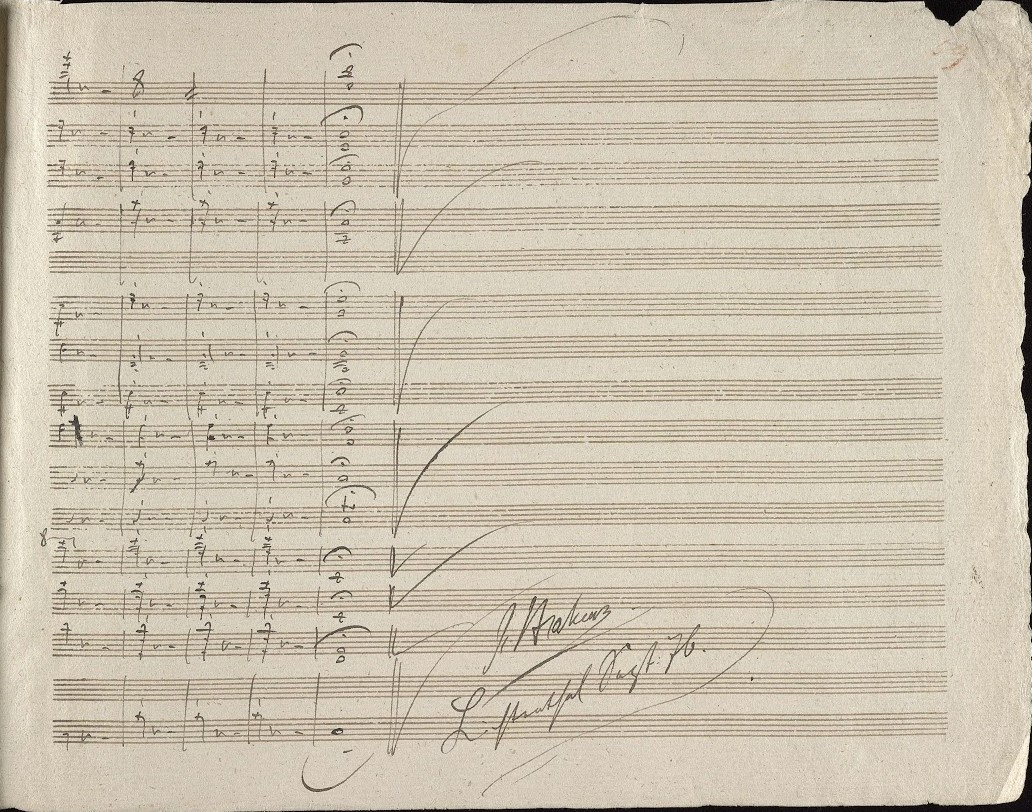
\includegraphics[clip,width=12.0cm]{./figure/mov4-59.jpg}
	\caption{自筆譜の最終ページ}
    \label{fig: mov4-59}
\end{figure}

\begin{figure}[htbp]
	\centering
    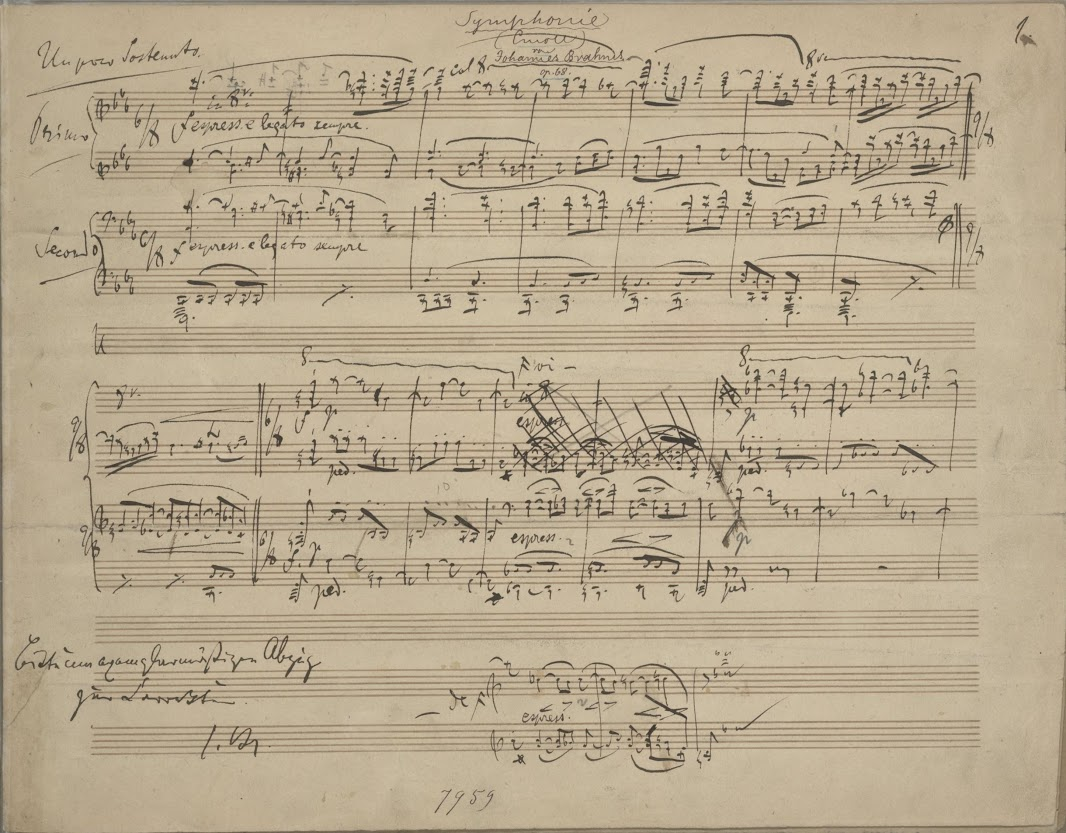
\includegraphics[clip,width=12.0cm]{./figure/mov1(4H)-01.jpg}
	\caption{ピアノ連弾版自筆譜の冒頭ページ}
    \label{fig: mov1(4H)-01}
\end{figure}
